% Artigo Lab03 — Métricas DORA em Repositórios Open-Source do GitHub
% Template SBC (sbc-template.sty / sbc-template.bst), PT-BR, ≤ 10 páginas com referências.
% Compile: pdflatex main && bibtex main && pdflatex main && pdflatex main

\documentclass[12pt]{article}

\usepackage{sbc-template}
\usepackage[brazil]{babel}
\usepackage[utf8]{inputenc}
\usepackage[T1]{fontenc}
\usepackage{graphicx}
\usepackage{booktabs}
\usepackage{hyperref}
\usepackage{amsmath}
\usepackage{url}

% Macros auxiliares
\newcommand{\pend}[1]{\textbf{[PENDENTE: #1]}}

\sloppy

\title{Métricas DORA em Repositórios Open-Source do GitHub:\\
uma análise exploratória de 300 projetos}

\author{Arthur Soares\inst{1} \and Guilherme Vieira\inst{1} \and Marcos Pinto\inst{1}}

\address{Departamento de Ciência da Computação\\
  Universidade Federal de Minas Gerais (UFMG) -- Belo Horizonte, MG, Brasil
  \email{\{arthur, guilherme, marcos\}@dcc.ufmg.br}
}

\begin{document}

\maketitle

\begin{abstract}
We present an exploratory analysis of DORA metrics (deployment frequency, lead time for
changes, change failure rate and mean time to recovery) mined from 300 popular open-source
GitHub repositories. Using releases as a deploy proxy and CI workflow failures as a
production failure proxy, we find a median deployment frequency of 0.36 releases/week
(Medium tier), median lead time of 146~h ($\approx$ 6 days), median CI failure rate of
5.7\%, and median recovery time of 2.8~h. A corrective-release heuristic (v12, F1 = 0.689)
provides an alternative CFR proxy, with a surprisingly strong positive Spearman correlation
with deployment frequency ($\rho = 0.62$, $p < 0.001$), contradicting the DORA ``no
trade-off'' thesis for this proxy. Classification sensitivity to the operational definition
of deploy changes 22--40\% of repositories across combinations, with linear kappa between
0.46 and 0.72.
\end{abstract}

\begin{resumo}
Apresentamos uma análise exploratória das métricas DORA (\textit{deployment frequency},
\textit{lead time for changes}, \textit{change failure rate} e tempo de recuperação) obtidas
de 300 repositórios open-source populares no GitHub. Usando \textit{releases} como proxy de
deploy e falhas de CI como proxy de falha em produção, encontramos frequência mediana de
0,36 releases/semana (nível \textit{Medium}), \textit{lead time} mediano de 146~h
($\approx$ 6 dias), CFR(a) mediano de 5,7\% e tempo de recuperação mediano de 2,8~h.
Uma heurística de releases corretivas (v12, F1 = 0,689) oferece um proxy alternativo de
CFR com correlação de Spearman positiva forte com a frequência de deploy ($\rho = 0{,}62$,
$p < 0{,}001$), contrariando a tese DORA de ausência de \textit{trade-off} para esse proxy.
A sensibilidade da classificação DORA à definição operacional de deploy altera a categoria
de 22--40\% dos repositórios entre as combinações testadas, com kappa linear entre 0,46 e
0,72.
\end{resumo}

% Introdução (versão compacta para o limite de 10 páginas). Versão completa: artigo/completo/introducao.tex.
% As hipóteses foram escritas ANTES de qualquer análise (Issue #15, Lab03S01); aqui só foram condensadas, sem
% mudar a expectativa de cada uma. A redação original está em artigo/completo/introducao.tex.
\section{Introdução}

As métricas DORA (\textit{DevOps Research and Assessment}) tornaram-se o padrão de mercado para medir o
desempenho de entrega de software~\cite{forsgren2018accelerate}. Quatro medidas descrevem duas dimensões:
velocidade (\textit{deployment frequency} e \textit{lead time for changes}) e estabilidade (\textit{change failure
rate} e tempo de recuperação). O relatório \textit{Accelerate State of DevOps} sustenta que as melhores equipes
vão bem nas duas dimensões, isto é, que velocidade e estabilidade não são um \textit{trade-off}.

O GitHub não registra ``deploys em produção'' nem ``falhas em produção''; só é possível \emph{inferir} as métricas
por \textbf{proxies}: uma \textit{release} publicada faz o papel de deploy, e uma execução de CI que falhou, o de
falha. Por isso cada métrica minerada precisa de uma medida de confiança. Este trabalho \textbf{calcula as métricas DORA} de repositórios populares que usam GitHub Actions e
\textbf{mede o quanto as conclusões dependem das definições operacionais}. Hipóteses informais, escritas antes
de ver os dados:

\begin{description}\setlength{\itemsep}{1pt}
  \item[H1 (RQ01).] Distribuição muito assimétrica, com mediana entre uma \textit{release} a cada duas semanas e
  uma por mês (\textit{Medium}) e cauda de projetos com mais de uma por semana.
  \item[H2 (RQ02).] A mediana por commit (b) será bem menor que a por \textit{release} (a), pois um commit antigo
  incluído na \textit{release} faz (a) crescer e afeta pouco (b); \textit{lead times} medianos de semanas a poucos meses.
  \item[H3 (RQ03).] O CFR (a), de CI, será maior que o (b), de \textit{releases} corretivas, com mediana de (a) entre
  10\% e 30\%: falhas de pipeline são comuns e raramente chegam a uma \textit{release} corretiva.
  \item[H4 (RQ04).] A maioria dos episódios se resolve em horas, com cauda longa; mediana por repositório entre 1 hora
  e 1 dia, e parcela relevante de episódios censurados.
  \item[H5 (RQ05).] Correlação de Spearman fraca ou levemente negativa entre frequência e CFR, em linha com a tese
  DORA, mas com ruído por causa dos proxies.
  \item[H6 (RQ06).] Linguagem e tipo de projeto terão associação mais forte que a popularidade; aplicações publicam
  mais que bibliotecas; idade e contribuidores terão efeitos pequenos, e a maioria das diferenças perderá
  significância após a correção para comparações múltiplas.
  \item[H7 (RQ07).] Mais de 30\% dos repositórios mudarão de categoria ao trocar a definição de deploy e as variantes
  de LT e CFR, com $\kappa$ ponderado no máximo moderado.
\end{description}


% Metodologia do artigo (template SBC) — Lab03S02, Issue #31. RASCUNHO baseado só em artefatos do repositório.
% Cada afirmação factual aponta a fonte em comentário (%). Itens que dependem do professor aparecem como
% \pend{...}; decisões provisórias do grupo como \prov{...}. Evidências e lacunas: docs/metodologia_evidencias.md.
\newcommand{\pend}[1]{\textbf{[PENDENTE DO PROFESSOR: #1]}}
\newcommand{\prov}[1]{\textbf{[PROVISÓRIO: #1]}}

\section{Metodologia}

\subsection{Questões de pesquisa e desenho do estudo}
% E§5; fonte_vdd.md
O estudo é observacional e mineratório: calcula as métricas DORA a partir de dados públicos do GitHub
(\textit{releases}, \textit{commits} e execuções de GitHub Actions) de repositórios open-source. As
questões de pesquisa seguem o enunciado: RQ01 frequência de deploy; RQ02 \textit{lead time} (variantes
por \textit{release} e por \textit{commit}); RQ03 \textit{change failure rate} (variante (a), proxy de CI,
e (b), proxy de entrega); RQ04 tempo de recuperação; RQ05 correlação entre frequência e CFR; RQ06
características associadas ao desempenho; RQ07 sensibilidade da classificação DORA à definição operacional.
Como o GitHub não registra deploys nem falhas em produção, todas as medidas são \emph{proxies}.
Esta seção descreve a coleta e a validação manual; as análises estatísticas das RQ01--RQ07 pertencem à
Sprint~3 e \textbf{ainda não foram executadas}.

\subsection{Seleção dos repositórios e funil}
% outputs/funil.md, config.yaml (selecao:)
Os candidatos vieram da Search API, fatiada por faixas de estrelas a partir de 1000 (\texttt{stars:>=1000},
sem forks e sem repositórios arquivados). \prov{o enunciado não define ``popular''; o piso de 1000 estrelas,
a exclusão de forks/arquivados e as faixas de fatiamento são decisão do grupo (lacuna L03)}.
Critérios de inclusão (E§3): uso de GitHub Actions, ao menos 5 \textit{releases} e ao menos 50
\textit{workflow runs} válidos no \textit{default branch} dentro da janela. \prov{a leitura de ``run válido''
(\texttt{event=push}, criado na janela, \texttt{conclusion} em \{success, failure, timed\_out,
startup\_failure\}) e a de ``release contada'' (não rascunho, não pré-release, publicada na janela) são
interpretações do grupo (L04, L05)}.

\begin{table}[ht]
\centering
\caption{Funil de seleção (\texttt{outputs/funil.csv}).}
\begin{tabular}{lrrr}
\hline
Etapa & Entram & Saem & Restam \\ \hline
Candidatos avaliados (sem duplicatas) & 2677 & --- & 2677 \\
Possui Actions & 2677 & 1219 & 1458 \\
Releases mínimas (5) & 1458 & 1038 & 420 \\
Runs válidos mínimos (50) & 420 & 120 & 300 \\
Amostra final & 300 & --- & 300 \\ \hline
\end{tabular}
\end{table}

A Search API devolveu 60\,143 resultados brutos (60\,142 após deduplicação), dos quais 2677 foram
avaliados em ordem determinística por \texttt{full\_name}; a avaliação parou ao atingir 300 repositórios,
e 57\,465 candidatos \emph{não foram avaliados}. Assim, a amostra não é aleatória sobre a população de
candidatos: é o primeiro conjunto de 300 que passa nos filtros nessa ordem (lacuna L17, corte não definido
pelo enunciado). O relatório marca todas as fatias como não saturadas, mas a fatia \texttt{stars:1282..1312} tem
exatamente 1000 resultados (o teto da API); \pend{confirmar se esse caso foi truncado}.

\subsection{Janela temporal}
% config.yaml (L01); data/amostra_ouro/sorteio.json
A janela de 12 meses usada nos artefatos atuais é 2025-10-02 a 2026-10-02 (UTC). \pend{as datas oficiais
da janela não constam do material fornecido (lacuna L01); o \texttt{config.yaml} as declara
\emph{provisórias}. Se mudarem, seleção, coleta e sorteio da amostra-ouro precisam ser refeitos}.

\subsection{Definições operacionais das métricas}
% E§3, E§5; metricas/*.py; README
Valem as definições comuns do enunciado: deploy é uma \textit{release} publicada (\texttt{draft=false},
sem pré-release na definição principal); a data de um \textit{commit} é \texttt{commit.author.date};
considera-se apenas o \textit{default branch} para execuções de CI, com \texttt{event=push}; a
classificação de falha/sucesso segue a tabela de \texttt{conclusion} do enunciado, ignorando
\texttt{cancelled}, \texttt{skipped}, \texttt{neutral}, \texttt{action\_required}, \texttt{stale} e execuções
em andamento.
\begin{itemize}
  \item \textbf{Deployment frequency:} \textit{releases} publicadas na janela dividido pelo número de
  semanas da janela (RQ01).
  \item \textbf{Lead time (a)/(b):} por \textit{release}, \texttt{publicação $-$ commit mais antigo}; por
  \textit{commit}, \texttt{publicação $-$ data do commit}; mediana por repositório, em horas. Commits
  vêm de \texttt{compare/\{anterior\}...\{R\}}; a primeira \textit{release} da história é ignorada, e
  \textit{releases} com \texttt{compare} 404 também. \prov{releases sem commits novos e commits com data
  posterior à release são excluídos (L07)}.
  \item \textbf{CFR (a):} falhas $\div$ (falhas $+$ sucessos) das execuções de CI.
  \item \textbf{CFR (b):} uma \textit{release} R falha se qualquer \textit{release} de deploy em
  $(R, R{+}7\text{d}]$ for corretiva; \textit{releases} nos últimos 7 dias da janela ficam fora do
  denominador (censura); com menos de 2 \textit{releases} na janela o valor é indefinido.
  \prov{``qualquer release no intervalo'', e não só a próxima, é decisão do grupo (L08)}.
  \item \textbf{Tempo de recuperação:} por workflow, do início da primeira falha após um sucesso até o fim
  (\texttt{updated\_at}) do próximo sucesso; mediana por repositório; episódios sem fim na janela são
  censurados e reportados em proporção.
  \item \textbf{Classificação DORA:} cortes fixos adaptados pelo enunciado (Elite/High/Medium/Low) e
  mediana arredondada para baixo das quatro notas.
\end{itemize}
O CFR (b) \textbf{não} está no arquivo de métricas atual (\texttt{outputs/resultados.csv}): a coluna
\texttt{cfr\_b} não existe nele, porque a heurística não foi validada (Seção~\ref{sec:heuristica}).

\subsection{Procedimento de coleta, cache e limitações da API}
% README; pipeline/http_client.py; outputs/execucao.log, funil.md
A coleta é feita por script próprio, via API REST, sem bibliotecas de acesso ao GitHub. Cada resposta é
armazenada em disco e a execução é retomável: o último \textit{run} registrado em
\texttt{outputs/execucao.log} processou 300 repositórios sem erros, com 12\,191 acertos e 72\,975 falhas de
cache (execução iniciada em 2026-10-11). O cliente espera o \textit{rate limit} renovar (até 10 esperas por
requisição) e repete erros 5xx com \textit{backoff} exponencial (1, 2, 4, 8~s, até 5 tentativas).
Limitações conhecidas: (i) a Search API devolve no máximo 1000 resultados por consulta, por isso a busca é
fatiada; (ii) execuções de CI são coletadas por mês, e nenhum dia atingiu o teto de 1000 resultados
(\texttt{n\_runs\_dias\_saturados} $=0$ em todos os repositórios de \texttt{resultados.csv}); (iii) o
\texttt{compare} é paginado; (iv) \textit{releases} com \texttt{compare} divergente (backports) mantêm
os commits desde o \textit{merge-base} e podem inflar o \textit{lead time}; (v) o cache não é versionado,
portanto a coleta só é reproduzível por quem o possui ou refaz as chamadas, e \emph{repositórios continuam
recebendo commits}, de modo que uma nova coleta pode divergir.

\subsection{Rotulagem manual, sugestões assistidas e consenso}
% data/amostra_ouro/{sorteio.json,LEIAME.md,PROTOCOLO_CONSENSO.md,consenso.csv}; rascunho/revisao_*.csv
Foram sorteados 60 repositórios da lista de entrada \texttt{resultados.csv} (semente 42; \texttt{sha256}
registrado em \texttt{sorteio.json}) e 5 \textit{releases} por repositório (300 \textit{releases}, as
mesmas para os três avaliadores). Cada avaliador preencheu, em arquivo próprio, (i) o tipo do projeto,
(ii) se as \textit{releases} são entregas reais e (iii) se cada \textit{release} é corretiva.

\textbf{Uso de sugestões.} A rotulagem usou sugestões: \texttt{scripts/rotular.py} apresenta notas e
commits de cada item junto de uma \emph{sugestão}, igual para todos os avaliadores, que o avaliador aceita
ou substitui. Existem 292 sugestões para os 300 itens de \texttt{corretiva} (71 ``sim'', 221 ``não''); os
8 restantes ficaram sem sugestão.

\textbf{Rodada anterior (rótulos que não são os commitados).} Numa primeira rodada, feita com versões dos
arquivos de rótulos que não foram as commitadas, os arquivos de revisão de \textbf{dois} avaliadores
(guardados fora do Git) coincidiam com a sugestão em \textbf{292/292} itens, esses dois avaliadores
coincidiam entre si em 293 dos 300 itens (97,7\%) e o terceiro coincidia com a sugestão em 181 dos 292
(62,0\%).

\textbf{Arquivos commitados (usados nos resultados abaixo).} Os rótulos oficiais são os três
\texttt{labels\_<avaliador>.csv} commitados nas Issues \#23, \#24 e \#25. Neles, a concordância em
\texttt{corretiva} é de 82,0\% (246/300) entre ALuiz19 e marcosffp, 63,3\% (190/300) entre ALuiz19 e
GuilhermeVieira05 e 56,0\% (168/300) entre GuilhermeVieira05 e marcosffp. A aderência desses arquivos à
sugestão não pode ser recalculada, porque \texttt{sugestoes.csv} e os arquivos de revisão estão fora do Git.

Não há, nos artefatos, registro de como as sugestões foram geradas (\texttt{sugestoes.csv} traz só rótulo
e motivo textual). Os fatos acima não permitem concluir que os rótulos estejam errados: uma sugestão
pode estar correta. Eles apenas \emph{não demonstram} três julgamentos independentes, e o critério de
independência do enunciado (``sem consultar os demais'') não é verificável nesses casos.

\textbf{Repositório removido.} O repositório \texttt{1bananachicken/MaaNTE} (5 \textit{releases} da
amostra) foi removido do GitHub depois do sorteio: a API devolve 404 para o repositório, as
\textit{releases}, os \texttt{compare} e a conta do dono. Ele foi mantido na amostra por decisão do grupo.
Dois dos três avaliadores rotularam essas \textit{releases} sem acesso ao conteúdo (registrado na coluna
\texttt{observacoes}).
\pend{se a rotulagem assistida é metodologicamente aceitável para a validação, ou se a amostra deve ser
rotulada de novo sem sugestões, é decisão do professor}.

O protocolo de consenso (\texttt{PROTOCOLO\_CONSENSO.md}) é: unanimidade; maioria simples em 2 a 1;
reunião para 1-1-1. O protocolo prevê o kappa antes do consenso. Resultado em \texttt{consenso.csv}:
\texttt{corretiva}, 152 por unanimidade e 148 por maioria (85 corretivas, 215 não); tipo do projeto, 44 e
16; entrega real, 55 e 5; nenhum caso \texttt{reuniao} nem \texttt{pendente}.

\subsection{Concordância entre avaliadores}
% data/amostra_ouro/concordancia.csv; recalculado a partir de labels_*.csv com statsmodels
\begin{table}[ht]
\centering
\caption{Kappa de Fleiss (3 avaliadores). Interpretação de Landis \& Koch.}
\begin{tabular}{lrrl}
\hline
Dimensão & Itens & $\kappa$ & Interpretação \\ \hline
Tipo do projeto & 60 & 0,743 & substancial \\
Releases são entregas reais & 60 & 0,352 & razoável \\
Release corretiva & 300 & 0,273 & razoável \\ \hline
\end{tabular}
\end{table}
O kappa baixo da dimensão \texttt{corretiva} indica que o próprio critério é ambíguo, o que é um achado e
limita qualquer validação contra esse consenso. A concordância simples foi 0,507 em \texttt{corretiva}.
Em \texttt{entrega real}, a concordância simples é alta (0,917), mas quase todos os rótulos são ``sim'',
o que derruba o kappa (efeito de prevalência).
\textbf{Limitação na leitura do kappa.} O kappa de Fleiss pressupõe avaliações independentes, o que os
artefatos não demonstram (ver acima). Com a maioria 2 a 1, o par de avaliadores mais próximo (82,0\% de
concordância em \texttt{corretiva}) pesa mais no consenso do que o terceiro. Para a heurística, o consenso
usado como referência de precisão, \textit{recall} e F1 pode herdar o viés das sugestões; o sentido e a
magnitude desse efeito não foram medidos. Os valores foram calculados por \texttt{scripts.agreement} a
partir dos três arquivos commitados (\texttt{concordancia.csv}).
Outras medidas de avaliação usadas: precisão, \textit{recall} e F1 (\texttt{precision\_recall\_fscore\_support},
positivo = corretiva). Nenhum intervalo de confiança foi calculado. \pend{se o professor exige
intervalos de confiança ou outro teste para essas medidas, não há procedimento definido nos documentos}.

\subsection{Heurística de release corretiva: versões e desempenho}\label{sec:heuristica}
% data/amostra_ouro/avaliacao_heuristica.csv; docs/refino_heuristica.md; git log
A heurística v1 reproduz o exemplo do professor (``só muda o \textit{patch} e contém \texttt{fix}'') e foi
definida antes de ver os dados. As versões v2--v7 combinam os mesmos dois sinais (SemVer e palavra-chave,
estrita ou ampla). As versões v8 e v9 olham o \emph{conteúdo} (commits de correção e de feature; na v9,
também as \textit{release notes}) e foram desenhadas \textbf{depois} de analisar os erros da v1--v7 na
\emph{mesma} amostra em que são avaliadas. Além disso, v8 e v9 entraram no repositório (PR \#65, 14/10,
21h19) \emph{antes} de os rótulos de dois avaliadores serem commitados (PRs \#67 e \#68, 21h46 e 21h59):
foram desenhadas sobre a rodada anterior de rótulos.

Cada versão é medida de duas formas: em todas as \textit{releases} em que ela é aplicável (300; a v9,
que exige as notas, em 295, porque as 5 \textit{releases} do repositório removido não têm notas) e no
\emph{subconjunto comum} às nove versões (295 \textit{releases}), usado para compará-las.

\begin{table}[ht]
\centering
\caption{Versões testadas contra o consenso (300 \textit{releases}; 85 corretivas). Precisão, \textit{recall}
e F1 em todas as \textit{releases} aplicáveis ($n$); F1 comum no subconjunto de 295. Fonte:
\texttt{avaliacao\_heuristica.csv}.}
\begin{tabular}{llrrrrrl}
\hline
Versão & Regra & $n$ & Precisão & Recall & F1 & F1 comum & Desenho \\ \hline
v1 & patch \textbf{e} palavra estrita & 300 & 0,423 & 0,741 & 0,539 & 0,546 & antes dos dados \\
v2 & patch \textbf{ou} palavra estrita & 300 & 0,329 & 0,988 & 0,494 & 0,485 & antes da análise de erros\textsuperscript{*} \\
v3 & só palavra estrita & 300 & 0,313 & 0,835 & 0,455 & 0,460 & idem\textsuperscript{*} \\
v4 & só patch (não comparável: palavra) & 300 & 0,429 & 0,894 & 0,580 & 0,570 & idem\textsuperscript{*} \\
v5 & patch \textbf{e} palavra ampla & 300 & 0,432 & 0,788 & 0,558 & 0,565 & idem\textsuperscript{*} \\
v6 & patch \textbf{ou} palavra ampla & 300 & 0,328 & 0,988 & 0,493 & 0,484 & idem\textsuperscript{*} \\
v7 & só palavra ampla & 300 & 0,321 & 0,882 & 0,470 & 0,475 & idem\textsuperscript{*} \\
v8 & correção e nenhuma feature & 300 & 0,625 & 0,412 & 0,497 & 0,507 & depois da análise de erros \\
v9 & v8 \textbf{ou} notas com correção e sem novidade & 295 & 0,627 & 0,573 & 0,599 & 0,599 & depois da análise de erros \\ \hline
\end{tabular}
\par{\footnotesize \textsuperscript{*} v2--v7 entraram no mesmo \textit{commit} do script de avaliação
(\texttt{360adc7}), antes dos arquivos de resultado; a ordem exata entre escrevê-las e a primeira rodada
não é verificável pelo histórico.}
\end{table}

\textbf{Status: heurística não validada.} O critério do enunciado é F1 $\geq$ 0,70, e o melhor F1 observado
foi 0,599 (v9, $n$ = 295); entre as versões aplicáveis a todo o \textit{dataset}, o melhor foi 0,580 (v4).
Conforme o enunciado, as versões e o F1 de cada uma são documentados aqui. A coluna
\texttt{escolhida} de \texttt{avaliacao\_heuristica.csv} é apenas a regra interna do script (maior F1 comum
quando ninguém atinge 0,70) e \emph{não} indica validação. \prov{o grupo adotou v8 como estimativa exploratória do
CFR (b), v4 como sensibilidade e v9 fora do dataset final (\texttt{docs/refino\_heuristica.md})}; com os
rótulos commitados, porém, a v8 (F1 0,497) ficou abaixo da v4 (0,580) e da v5 (0,558), e essa estratégia
precisa ser revista pelo grupo. A v9
depende das \textit{release notes} (\texttt{body}), que a coleta atual não armazena; por isso ela só foi
aplicada à amostra-ouro, onde as notas foram buscadas à parte. \pend{o enunciado e a Fonte da Verdade
não dizem como proceder se nenhuma versão chegar a F1 $\geq$ 0,70, nem se o CFR (b) exploratório é
aceitável; também não definem amostra independente para validação final}.

\subsection{Dados ausentes, censura e ameaças à validade}
% outputs/resultados.csv (contagem direta); E§3, E§5, E§11
\textbf{Dados ausentes e censura.} Casos censurados não são descartados: dos 9062 episódios de falha
em \texttt{resultados.csv}, 176 foram censurados; 6 \textit{releases} foram ignoradas no \textit{lead
time} por 404 no \texttt{compare}; 23 repositórios têm tempo de recuperação indefinido (sem episódios
concluídos). \prov{a mediana de recuperação usa só episódios concluídos e a proporção de censurados é
reportada à parte (L09)}. No CFR (b), \textit{releases} dos últimos 7 dias da janela ficam fora do
denominador. Em \texttt{resultados.csv}, 381 commits (32 repositórios) foram excluídos do \textit{lead time} por data posterior à release e 1685 \textit{releases} (51 repositórios) não têm commits novos (\texttt{python -m scripts.data\_quality}). Cinco \textit{releases} da amostra-ouro têm mensagens incompletas (\texttt{compare} 404 ou
truncado), o que pode ocultar a palavra-chave.

\textbf{Ameaças à validade} (resumo; a seção completa é entregue com o artigo final):
\begin{itemize}
  \item \emph{Construto:} \textit{release} $\neq$ deploy; falha de CI $\neq$ falha em produção;
  \textit{commit} com \textit{rebase}/\textit{squash} distorce a data; \textit{releases} não são
  filtradas pelo \textit{default branch}; a heurística corretiva não é validada.
  \item \emph{Interna:} v8/v9 foram desenhadas sobre a amostra em que são avaliadas, antes de os rótulos
  oficiais de dois avaliadores serem commitados, e a escolha é feita entre nove versões, o que torna o F1
  otimista; a rotulagem assistida reduz a independência dos avaliadores; um repositório da amostra foi
  removido e rotulado sem acesso ao conteúdo por dois avaliadores.
  \item \emph{Externa:} amostra dos primeiros 300 repositórios que passam nos filtros em ordem
  alfabética, com piso de 1000 estrelas; não representa projetos corporativos nem a população de
  candidatos.
  \item \emph{Conclusão:} kappa razoável (0,273) em \texttt{corretiva}; a amostra-ouro tem 60 repositórios e
  5 \textit{releases} por repositório; \textbf{nenhuma análise estatística das RQs foi feita até aqui}.
\end{itemize}


% Resultados e Discussão (versão compacta para o limite de 10 páginas). Versão completa: artigo/completo/resultados.tex.
% TODOS os números vêm de macros \N... (artigo/gerado/numeros.tex) e das tabelas de artigo/gerado/, geradas por
% `python -m analysis.artigo_numeros` a partir de outputs/analise/ e outputs/sensitivity_dora.csv, regenerados de
% data/metrics.csv (tag dataset-final). Não digitar números aqui. Conferência: `python -m analysis.artigo_numeros --check`.

\section{Resultados e Discussão}\label{sec:resultados}

Todas as análises partem de \texttt{data/metrics.csv} ($n = \NTotal$ repositórios) e reportam mediana e IQR,
com os cortes fixos da disciplina (Tabela~\ref{tab:resumo}). Release $\neq$ deploy e falha de CI $\neq$ falha em
produção; o CFR~(b) é \textbf{exploratório}, pois a heurística obteve F1 independente de 0,689, abaixo da meta de 0,70
(Seção~\ref{sec:heuristica}). A Tabela~\ref{tab:hipoteses} confronta as hipóteses da Introdução com os resultados.

\begin{table}[ht]
\centering\footnotesize
\caption{Mediana, quartis, IQR e classe DORA por métrica. ``Classe'' classifica a mediana; E/H/M/L são os
repositórios em Elite/High/Medium/Low. Recuperação: só repositórios com episódio concluído.}
\label{tab:resumo}
\resizebox{\linewidth}{!}{% Gerado por analysis/artigo_numeros.py a partir de outputs/analise/rq01_rq04_descritiva.csv. Não editar.
\begin{tabular}{llrrrrrll}
\hline
RQ & Métrica & $n$ & Mediana & Q1 & Q3 & IQR & Classe (mediana) & E/H/M/L \\ \hline
RQ01 & Deployment frequency (rel./sem.) & 300 & 0{,}36 & 0{,}19 & 0{,}77 & 0{,}58 & Medium & 6/55/143/96 \\
RQ02 & Lead time (a), por release (h) & 300 & 146{,}4 & 26{,}8 & 544{,}4 & 517{,}6 & High & 70/88/86/56 \\
RQ02 & Lead time (b), por commit (h) & 300 & 146{,}3 & 32{,}5 & 437{,}0 & 404{,}6 & High & 66/87/95/52 \\
RQ03 & CFR (a), proxy de CI (\%) & 300 & 5{,}7 & 2{,}4 & 14{,}1 & 11{,}7 & Elite & 229/40/17/14 \\
RQ03 & CFR (b), proxy de entrega (\%) & 299 & 20{,}0 & 4{,}1 & 46{,}5 & 42{,}4 & High & 121/67/33/78 \\
RQ04 & Recuperação (h) & 277 & 2{,}8 & 0{,}7 & 21{,}2 & 20{,}6 & High & 92/126/43/16 \\
\hline
\end{tabular}
}
\end{table}

\begin{table}[ht]
\centering\footnotesize
\caption{Hipóteses $\times$ resultados (expectativas na Introdução).}
\label{tab:hipoteses}
\begin{tabular}{@{}lp{11.2cm}l@{}}
\hline
\textbf{H} & \textbf{Observado (a expectativa está na Introdução)} & \textbf{Confirmada?} \\
\hline
H1 & Mediana \NDfMed{} rel./sem.; \NDfClasseHigh\% \textit{High} e \NDfClasseElite\% \textit{Elite} & Sim \\
H2 & Medianas iguais (\NLtaMed{} h e \NLtbMed{} h); por repositório, razão LT(a)/LT(b) com mediana \NRazMed{} (IQR \NRazQum--\NRazQtres) & Não \\
H3 & CFR(a) \NCfraMed\%; CFR(b) \NCfrbMed\% & Não \\
H4 & Mediana \NRecMed{} h; censurados: \NCensPct\% dos episódios & Parcial \\
H5 & CFR(a): $\rho = \NRhoA$; CFR(b): $\rho = \NRhoB$ & Parcial \\
H6 & \NSeisSig{} de \NSeisTestes{} testes significativos: idade (4), contribuidores (2), linguagem (2), efeito médio; tipo e popularidade, nenhum & Parcial \\
H7 & C1$\times$C2: \NSensUmDoisPct\%, $\kappa = \NSensUmDoisKappa$; C1$\times$C3: \NSensUmTresPct\%, $\kappa = \NSensUmTresKappa$ & Parcial \\
\hline
\end{tabular}
\end{table}

\begin{figure}[ht]
\centering
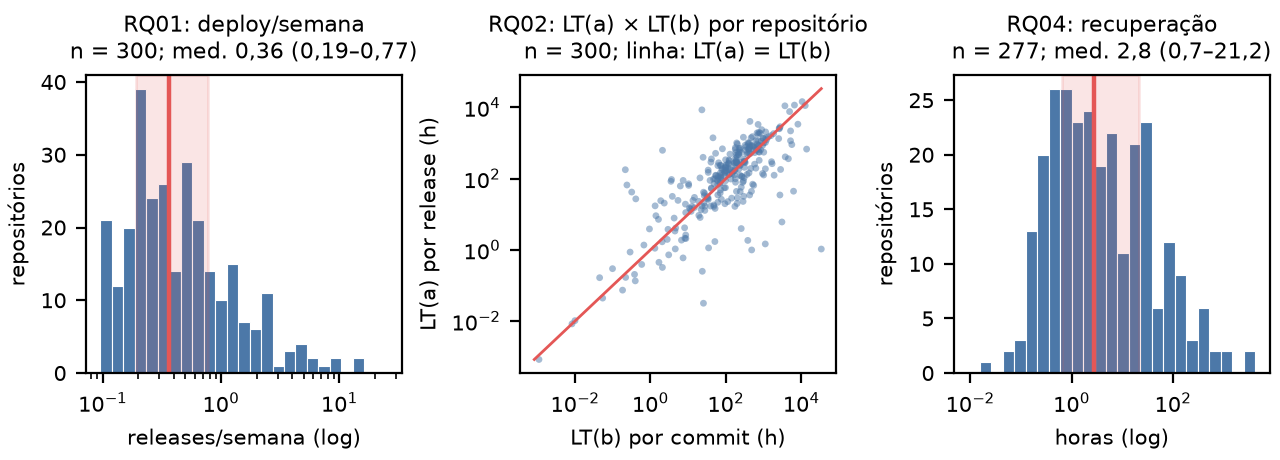
\includegraphics[width=\linewidth]{figs/fig_rq01_rq02_rq04.png}
\caption{RQ01, RQ02 e RQ04 por repositório (escala log). Linha e faixa vermelhas: mediana e IQR.}
\label{fig:rq124}
\end{figure}

\subsection{RQ01 --- Frequência de deploy}
A mediana foi de \textbf{\NDfMed{} releases/semana} (Q1 = \NDfQum; Q3 = \NDfQtres), pouco mais de uma \textit{release}
a cada três semanas, com cauda à direita (Figura~\ref{fig:rq124}). Pelos cortes da disciplina, \NDfClasseElite\%
são \textit{Elite}, \NDfClasseHigh\% \textit{High}, \NDfClasseMedium\% \textit{Medium} e \NDfClasseLow\% \textit{Low};
a classe geral C1 é \NUmClasseElite/\NUmClasseHigh/\NUmClasseMedium/\NUmClasseLow\% (E/H/M/L). A H1 se confirma.

\subsection{RQ02 --- Lead time for changes}
As medianas entre repositórios são \textbf{\NLtaMed{} h} para LT(a) ($\approx$ \NLtaDias{} dias; Q1 = \NLtaQum;
Q3 = \NLtaQtres) e \textbf{\NLtbMed{} h} para LT(b) (Q1 = \NLtbQum; Q3 = \NLtbQtres), ambas \textit{High}. Elas
coincidem, o que contraria a H2, mas só no agregado: por repositório a razão LT(a)/LT(b) tem mediana \NRazMed{} e
IQR \NRazQum--\NRazQtres; LT(a) supera o dobro de LT(b) em \NRazAdobroB\% dos repositórios, LT(b) supera o dobro de
LT(a) em \NRazBdobroA\% e só \NRazMeio\% ficam entre metade e o dobro (Wilcoxon pareado, $p$ \NRazWilcoxonP;
Figura~\ref{fig:rq124}). As variantes medem coisas diferentes: LT(a) usa o commit \emph{mais antigo} de cada
\textit{release}, e LT(b) pesa mais as \textit{releases} com muitos commits. Um commit antigo ``esquecido'' eleva
LT(a) sem mover muito LT(b), mas \NRazAmenorB\% dos repositórios têm LT(a) $<$ LT(b), o que ele não explica. Não
testamos causas: o lead time de cada commit está só no cache, não versionado.

\subsection{RQ03 --- Change failure rate}
O CFR~(a), proxy de CI, teve mediana de \textbf{\NCfraMed\%} (Q1 = \NCfraQum\%; Q3 = \NCfraQtres\%); o CFR~(b), proxy
de entrega, de \textbf{\NCfrbMed\%} (Q1 = \NCfrbQum\%; Q3 = \NCfrbQtres\%; $n = \NCfrbN$, pois um repositório tem menos
de duas \textit{releases} na janela). A H3 é refutada nos dois pontos. O CFR(a) conta \emph{execuções de CI} que
falharam, e falha de pipeline (teste instável, lint, ambiente) não é falha em produção; o CFR(b) conta
\textit{releases} seguidas de uma corretiva em 7 dias, segundo uma heurística imperfeita (F1 de 0,689), e mistura
correções reais com erros do proxy.

\subsection{RQ04 --- Tempo de recuperação}\label{sec:resultados-rq04}
A mediana foi de \textbf{\NRecMed{} h} (Q1 = \NRecQum; Q3 = \NRecQtres; $n = \NRecN$), classe \textit{High}.
\textbf{Censura:} \NCensEp{} de \NCensTot{} episódios (\NCensPct\%) não terminaram na janela; entre os \NCensReposCom{}
repositórios com episódio, a mediana da proporção de censurados é \NCensRepoMed\% (Q3 = \NCensRepoQtres\%) e
\NCensReposAlgum{} têm ao menos um censurado. Os censurados não entram na mediana, mas são contados. Dos
\NRecSemValor{} repositórios sem valor, \NCensReposSem{} não tiveram episódio e \NCensSoCens{} só tiveram censurados,
o que tende a subestimar a recuperação, pouco dado o volume de censura. A H4 se confirma só em parte: a mediana está
entre 1 h e 1 dia, mas a censura é bem menor que a esperada.

\begin{figure}[ht]
\centering
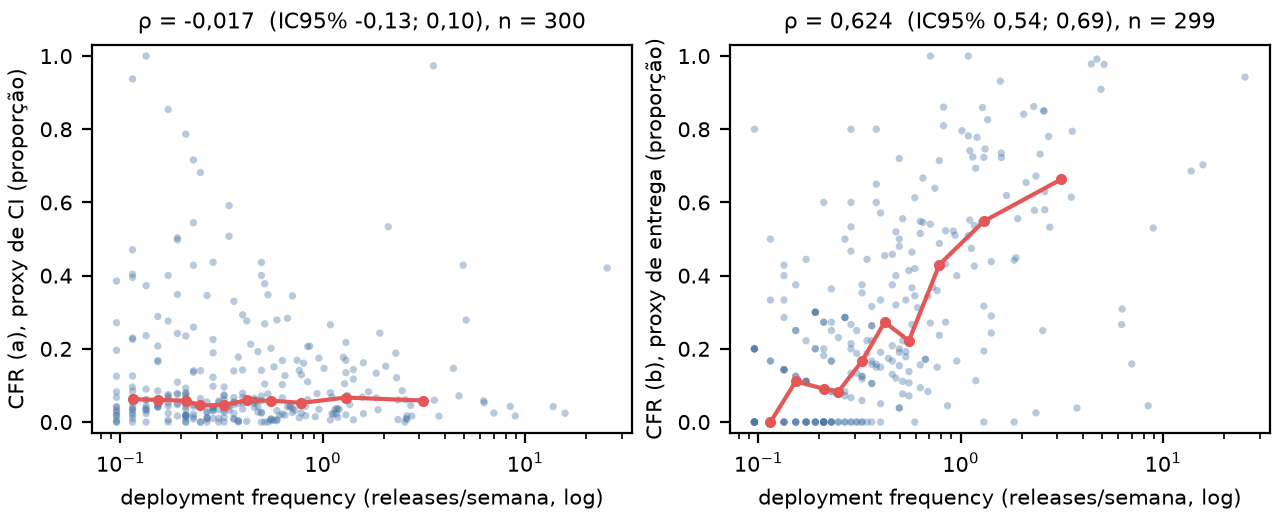
\includegraphics[width=\linewidth]{figs/fig_rq05.png}
\caption{RQ05: DF (escala log) $\times$ CFR(a) e CFR(b); linha vermelha: mediana do CFR por faixa de DF.}
\label{fig:rq05}
\end{figure}

\subsection{RQ05 --- Frequência de deploy $\times$ CFR}
Com o CFR(a), $\rho = \NRhoA$ ($p = $ \NRhoPA; IC 95\% \NRhoIcA; $n = \NRhoNA$): sem relação monotônica detectável.
Com o CFR(b), $\rho = \NRhoB$ ($p$ \NRhoPB; IC 95\% \NRhoIcB; $n = \NRhoNB$): correlação positiva forte
(Figura~\ref{fig:rq05}); os intervalos usam a transformação $z$ de Fisher com erro-padrão de Bonett e
Wright~\cite{bonett2000spearman}. A H5 se confirma só para (a). Isso não refuta a tese DORA, e correlação não implica
causalidade: o CFR(b) é acoplado mecanicamente à frequência (mais \textit{releases}, mais chances de uma corretiva em
7 dias), e com poucas \textit{releases} há muitos zeros. Com ao menos 20 \textit{releases} avaliadas, $\rho$ cai para
\NRhoBVinte{} ($n = \NRhoBVinteN$), mas isso também restringe a faixa de DF. A idade confunde (RQ06). O resultado (b) é um possível artefato, e o (a) é compatível com a tese.

\subsection{RQ06 --- Características dos repositórios}
Testamos cinco fatores (linguagem, popularidade, contribuidores, idade, tipo; $n = \NTipoN$ no tipo) contra as seis
métricas, \NSeisTestes{} testes. Todos os fatores têm três ou mais grupos, então todos usaram Kruskal-Wallis; Mann-Whitney
e o $\delta$ de Cliff~\cite{cliff1993dominance} (magnitude de Romano et al.~\cite{romano2006appropriate}) não foram
exercitados com dados reais, e o $\delta$ aparece só como contraste descritivo em \texttt{rq06\_testes.csv}. Os
p-valores foram corrigidos por Holm~\cite{holm1979sequentially} sobre os \NSeisTestes{} testes, e o efeito é
$\varepsilon^2 = H/(n-1)$, com a escala de Mangiafico~\cite{mangiafico2016handbook} (pequeno de $0{,}01$ a $<0{,}08$, médio até
$<0{,}26$; orientação do autor, não padrão; ``desprezível'' ($<0{,}01$) é rótulo nosso).
\textbf{\NSeisSig{} associações} permaneceram significativas, todas de efeito médio (Tabela~\ref{tab:rq06},
Figura~\ref{fig:rq06}). Os mais jovens (Q1 de idade) publicam mais (DF \NIdadeDfQum{} contra \NIdadeDfQquatro{}
rel./sem. no Q4), têm LT(a) menor (\NIdadeLtaQum{} h contra \NIdadeLtaQquatro{} h) e CFR(b) maior (\NIdadeCfrbQum\%
contra \NIdadeCfrbQquatro\%), em linha com o acoplamento da RQ05; mais contribuidores, LT(a) maior (\NContribLtaQum{} h
no Q1 contra \NContribLtaQquatro{} h no Q4); Rust tem os menores LT(a) e JavaScript a recuperação mais rápida. Popularidade (menor $p_{\mathrm{Holm}}$ = \NPopMinPHolm) e tipo não foram
significativos, e no tipo o $n$ limita o poder. A H6 é parcial: linguagem pesa mais que popularidade, mas o tipo não se
destaca, e idade e contribuidores têm efeito médio, não pequeno. São associações, não causas.

\begin{table}[ht]
\centering\footnotesize
\caption{RQ06: associações significativas após Holm (Kruskal-Wallis, $\varepsilon^2 = H/(n-1)$); os \NSeisTestes{} testes
estão em \texttt{outputs/analise/rq06\_testes.csv}.}
\label{tab:rq06}
\resizebox{\linewidth}{!}{% Gerado por analysis/artigo_numeros.py a partir de outputs/analise/rq06_testes.csv. Não editar.
\begin{tabular}{llrrrrl}
\hline
Fator & Métrica & $n$ & $H$ & $p_{\mathrm{Holm}}$ & $\varepsilon^2$ & Magnitude \\ \hline
Idade & Lead time (a) por release & 300 & 64{,}8 & $<0{,}001$ & 0{,}217 & médio \\
Idade & Lead time (b) por commit & 300 & 51{,}2 & $<0{,}001$ & 0{,}171 & médio \\
Idade & CFR (b) proxy de entrega & 299 & 40{,}3 & $<0{,}001$ & 0{,}135 & médio \\
Idade & Deployment frequency & 300 & 36{,}2 & $<0{,}001$ & 0{,}121 & médio \\
Contribuidores & Lead time (a) por release & 300 & 33{,}8 & $<0{,}001$ & 0{,}113 & médio \\
Contribuidores & Lead time (b) por commit & 300 & 26{,}0 & $<0{,}001$ & 0{,}087 & médio \\
Linguagem & Lead time (a) por release & 298 & 24{,}9 & $0{{,}}0087$ & 0{,}084 & médio \\
Linguagem & Tempo de recuperação & 276 & 22{,}2 & $0{{,}}025$ & 0{,}081 & médio \\
\hline
\end{tabular}
}
\end{table}

\begin{figure}[ht]
\centering
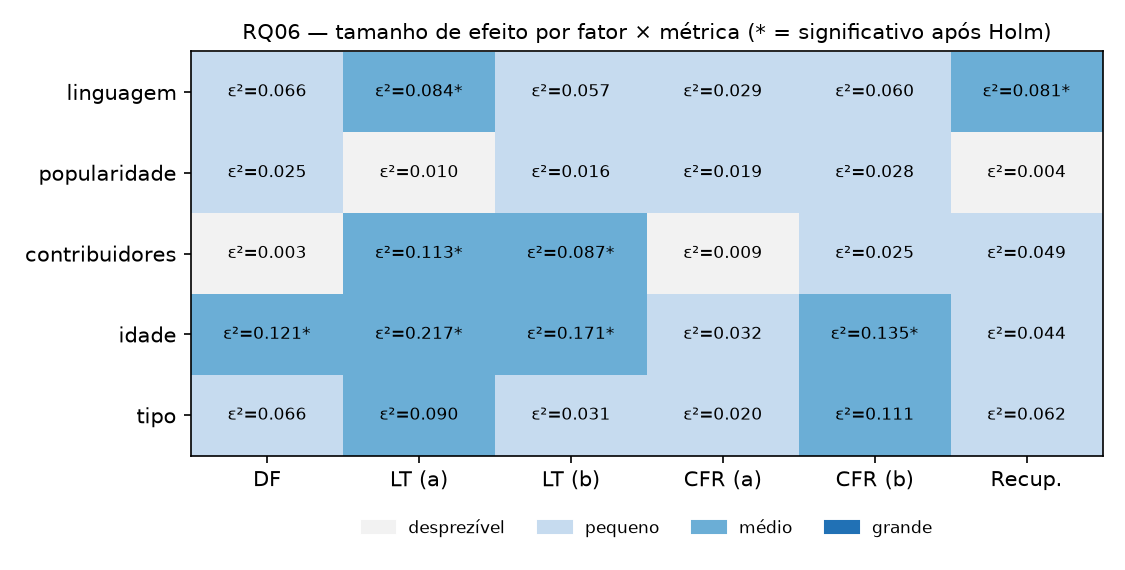
\includegraphics[width=.66\linewidth]{figs/rq06_efeitos.png}
\caption{RQ06: $\varepsilon^2$ por fator e métrica (* = significativo após Holm).}
\label{fig:rq06}
\end{figure}

\subsection{RQ07 --- Sensibilidade das classificações}
Comparamos C1 (release, LT(a), CFR(a)), C2 (release e pré-release, LT(b), CFR(b)) e C3 (tag, LT(b), CFR(a)), com
categorias codificadas de 1 a 4 e $\kappa$ linear ponderado~\cite{cohen1968weighted} (Figura~\ref{fig:rq07}).
C1$\times$C2 muda em \NSensUmDoisPct\% dos repositórios ($\kappa = \NSensUmDoisKappa$, moderado), o que confirma
a H7; C1$\times$C3 em \NSensUmTresPct\% ($\kappa = \NSensUmTresKappa$) e C2$\times$C3 em \NSensDoisTresPct\%
($\kappa = \NSensDoisTresKappa$), ambos substanciais, abaixo de 30\%. \textbf{Limitações:} em C2 e C3 só a unidade do DF
muda (LT(b) e CFR(b) seguem sobre releases), e \NParcialCUm, \NParcialCDois{} e \NParcialCTres{} repositórios em C1, C2 e C3
são classificados com três métricas.

\begin{figure}[ht]
\centering
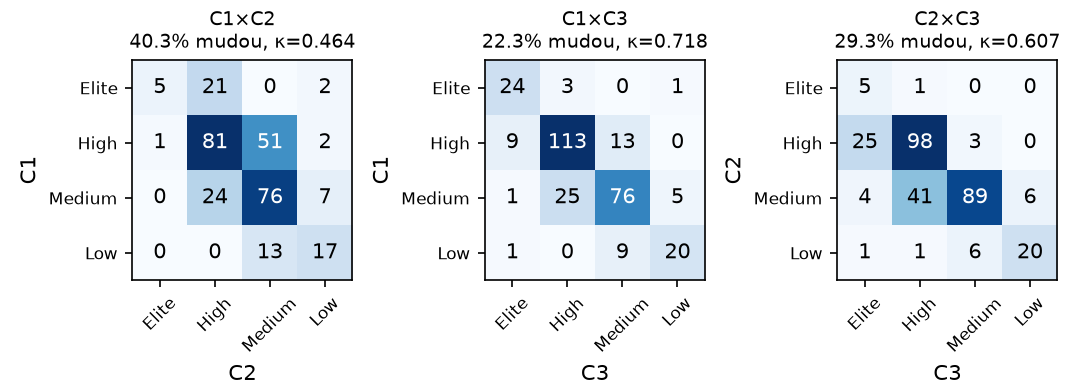
\includegraphics[width=.92\linewidth]{figs/sensitivity_transicao.png}
\caption{RQ07: matrizes de transição entre combinações (linha = primeira; coluna = segunda).}
\label{fig:rq07}
\end{figure}

\textbf{Robustez de RQ01--RQ06.} A maior discordância é C1$\times$C2, que troca CFR(a) por CFR(b) além da unidade de
deploy, coerente com as RQ03 e RQ05: as conclusões sobre CFR dependem da definição, e a de DF$\times$CFR(b) é a menos
robusta. As associações de LT da RQ06 aparecem em LT(a) e LT(b). A RQ01 depende da unidade de deploy (em C1$\times$C3,
\NSensUmTresPct\% mudam de classe), e a RQ04 não tem variante. Na análise ampliada, só quatro das sete variações
reclassificam de fato (janela do CFR(b) e cortes $\pm 10\%$): mudam \NAmpInfMinPct\% a \NAmpInfMaxPct\% dos repositórios,
com $\kappa \geq \NAmpInfKappaMin$; as outras três dão 0\% por construção e não são evidência de robustez. A classificação
é estável a pequenas perturbações dos cortes, mas depende da unidade de deploy e da variante de CFR.

\subsection{RQ08 --- Rework rate (bônus)}
A \textit{rework rate} (proporção de \textit{releases} corretivas) teve mediana de \textbf{\NRwMed\%} (Q1 = \NRwQum\%;
Q3 = \NRwQtres\%; $n = \NRwN$), contra \NRwCfrbMed\% do CFR(b) no subconjunto pareado. Três repositórios ficam fora (dois sem
rótulos no cache, um com contadores divergentes do \texttt{metrics.csv}). A diferença pareada
tem mediana 0, mas IQR de \NRwDifIqr{} p.p. e Wilcoxon $p = $ \NRwWilcoxonP; $\rho = \NRwSpearman$ entre as duas. As medidas
não são equivalentes: o CFR(b) conta a \textit{release} que \emph{precisou} de correção, e o rework a que \emph{é}
correção. Ambas herdam a imprecisão da heurística v12.


% Ameaças à validade — Lab03, Issue #49.
% Estrutura: 4 categorias de Wohlin et al. (2000) com evidências quantitativas do projeto.

\section{Ameaças à validade}

\subsection{Validade de construto}

\textbf{Release $\neq$ deploy.} A frequência de deploy e o \textit{lead time} são calculados a
partir de \textit{releases} publicadas no GitHub. Uma biblioteca que publica uma versão por mês
não ``faz deploy em produção''; quem faz isso são seus usuários. Repositórios de
infraestrutura ou de documentação podem não publicar nenhuma \textit{release} mesmo implantando
continuamente. Isso limita a generalização para projetos que adotam entrega contínua sem
\textit{releases} formais.

\textbf{Falha de CI $\neq$ falha em produção (CFR variante a).} O CFR(a) conta execuções de
CI com conclusão de falha; erros de lint, testes instáveis e falhas de ambiente não são
incidentes de produção. A mediana de 5,7\% pode subestimar (se falhas reais ficam ocultas)
ou superestimar (se a maioria das falhas não chega aos usuários).

\textbf{Heurística corretiva não validada (CFR variante b).} A v12 atingiu F1 = 0,689
(IC95\% 0,563--0,790) na amostra independente, abaixo da meta de 0,70. Toda conclusão
que use o CFR(b) — RQ03b, RQ05b e a combinação C2 da RQ07 — é exploratória. O $\kappa$
de Fleiss em \textit{corretiva} foi de 0,273 na amostra-ouro (razoável), o que indica que
a própria definição de ``release corretiva'' é ambígua para os avaliadores humanos.
As versões v8--v12 foram concebidas após examinar os erros da amostra de desenvolvimento,
tornando o F1 interno otimista.

\textbf{Rebase e squash distorcem a data do commit.} O \textit{lead time} usa
\texttt{commit.author.date} (E§3). Um rebase interativo altera a data do autor para o
momento do rebase, comprimindo artificialmente o LT para commits reorganizados. Não há
como detectar isso a partir da API pública.

\textbf{Releases fora do branch principal.} \textit{Releases} não são filtradas pelo
\textit{default branch}; backports publicados em ramos de manutenção entram no cálculo.
A contagem de \textit{releases} com \texttt{compare diverged} fica em
\texttt{n\_compare\_divergentes} no CSV.

\textbf{Correlação positiva DF × CFR(b) como artefato de denominador.} O coeficiente
$\rho = 0{,}62$ entre frequência de deploy e CFR(b) pode ser parcialmente explicado por
confundimento: projetos com muitas \textit{releases} têm mais oportunidades de publicar
correções, inflando o numerador do CFR(b) sem que isso reflita mais falhas reais.

\subsection{Validade interna}

\textbf{F1 otimista na escolha da heurística.} A versão escolhida (v12) foi selecionada
como a de maior F1 entre doze versões avaliadas na mesma amostra de desenvolvimento de
60 repositórios / 300 \textit{releases}. Sem um conjunto de validação separado, o F1
interno (0,722) é inflado; o F1 independente (0,689) é a estimativa mais confiável.

\textbf{Rotulagem assistida.} Os três avaliadores partilharam o protocolo de consenso e
discutiram desempates em reunião, o que reduz a independência real dos rótulos. O $\kappa$
de Fleiss por dimensão — 0,352 em ``entrega real'' e 0,273 em ``corretiva'' — indica
concordância razoável, mas aquém do que seria esperado em avaliadores verdadeiramente
independentes.

\textbf{Dados ausentes não aleatórios.} Os 23 repositórios sem tempo de recuperação
(nenhum episódio concluído) são projetos com poucas falhas de CI ou com episódios todos
censurados — possivelmente os mais estáveis da amostra. Excluí-los subestima o tempo
mediano de recuperação. Da mesma forma, os 2 repositórios sem CFR(b) são outliers de
comportamento incomum (\texttt{akto-api-security/akto}, com 1307 \textit{releases} avaliadas,
e \texttt{akveo/react-native-ui-kitten}, com 24 \textit{releases} todas censuradas).

\textbf{Censura no tempo de recuperação.} Episódios sem sucesso posterior até o fim da janela
são censurados e ficam fora da mediana. Se esses episódios são sistematicamente mais longos, a
mediana de 2,8~h subestima o tempo real de recuperação.

\subsection{Validade externa}

\textbf{Amostra por ordem alfabética com piso de estrelas.} Os 300 repositórios são os
primeiros que passam nos filtros (ações de CI, $\geq$ 5 \textit{releases}, $\geq$ 50 runs
válidos) em ordem alfabética dentro de faixas de estrelas com piso de aproximadamente 1000
estrelas. Isso exclui projetos menos populares e introduz viés de seleção: projetos com
nomes no início do alfabeto estão sobre-representados.

\textbf{Popularidade truncada.} O piso de popularidade garante que todos os repositórios
tenham alguma visibilidade, mas impede conclusões sobre projetos em estágio inicial ou de
nicho. Os resultados descrevem projetos open-source consolidados, não o ecossistema como um todo.

\textbf{Linguagens e tipos de projeto.} A amostra é dominada por TypeScript (22\%), Python
(18\%), Go (14\%) e Rust (10\%). Linguagens com ecosistemas de \textit{release} diferentes
(Java, PHP, Ruby) estão sub-representadas ou ausentes. O rótulo de tipo do projeto
(biblioteca, aplicação, CLI) está disponível apenas para os 60 repositórios da amostra-ouro.

\textbf{Janela de 12 meses.} A janela 2025-10-02 a 2026-10-02 captura um período específico;
projetos com ciclos de \textit{release} irregulares ou que mudaram de ritmo nesse intervalo
podem ter métricas não representativas do seu comportamento histórico.

\subsection{Validade de conclusão}

\textbf{Múltiplas comparações (RQ06).} A análise de fatores realiza 30 testes (5 fatores
$\times$ 6 métricas). A correção de Holm foi aplicada com $\alpha = 0{,}05$, e apenas 5
associações permaneceram significativas. Tamanhos de efeito medianos ($\eta^2_H$ entre 0,06
e 0,21) indicam que os fatores explicam pouca da variação total.

\textbf{Correlação de Spearman é monotônica, não linear.} O $\rho$ mede associação
monotônica; uma relação em U ou com limiar não seria detectada. A interpretação de
$\rho = 0{,}62$ entre DF e CFR(b) como ``correlação forte'' não implica causalidade nem
descarta formas funcionais não monotônicas.

\textbf{Número de testes por subgrupo.} Em RQ06, grupos com $n < 5$ foram excluídos.
O fator tipo do projeto tem apenas $n = 51$ repositórios com rótulo, contra $\approx$ 300
nos outros fatores, reduzindo o poder dos testes correspondentes.

\textbf{Sensibilidade à definição operacional (RQ07).} Entre 22\% e 40\% dos repositórios
mudam de categoria DORA ao trocar a combinação de métricas (C1, C2 ou C3), com $\kappa$
linear entre 0,46 e 0,72. Conclusões sobre a distribuição de níveis DORA dependem da
definição operacional escolhida, e comparações com outros estudos que adotem definições
diferentes devem ser feitas com cautela.


% Replicação cruzada — Lab03, Issue #49.
% Esta seção será preenchida após a conclusão das Issues #46 (execução do pipeline do outro
% grupo) e #47 (comparação e abertura de Issues no repositório do autor).

\section{Replicação cruzada}

\pend{Preencher após \#46 e \#47: grupo sorteado, commit fixo, SO/Python, n de repositórios
comparados, diferença relativa mediana por métrica, \% com mesma classe DORA, problemas
encontrados e Issues abertas.}


\section{Conclusão}

Este trabalho calculou as quatro métricas DORA para 300 repositórios open-source do GitHub
e respondeu sete questões de pesquisa. Os principais achados são: (i)~a maioria dos projetos
populares opera no nível \textit{Medium} ou \textit{High} de frequência de deploy, longe do
nível \textit{Elite}; (ii)~o \textit{lead time} por release e por commit são praticamente
idênticos (H2 refutada), sugerindo que commits chegam perto da data de publicação;
(iii)~o CFR por CI é baixo (5,7\%), mas o CFR por heurística corretiva é alto (20,0\%) e
positivamente correlacionado com a frequência de deploy, o que pode ser um artefato do
proxy; (iv)~as classificações DORA são sensíveis à escolha da unidade de deploy, o que
limita comparações entre estudos com definições operacionais distintas.

Como trabalhos futuros, sugerimos validar a heurística corretiva com uma amostra maior e
avaliadores independentes, explorar proxies que usem \textit{issues} e \textit{pull requests}
além de \textit{releases}, e replicar o estudo em repositórios privados ou corporativos.

\bibliographystyle{sbc}
\bibliography{referencias}

\end{document}
